\documentclass{parasim}
\usepackage{graphicx}
\usepackage{caption}
\usepackage{subcaption}

\title{Zpráva za období říjen až prosinec 2012}

\begin{document}

\section{Třetí etapa}

Ve druhé části třetí etapy, probíhající od začátku srpna do konce října, jsme se věnovali zejména
optimalizaci a paralelizaci výpočtu a implementaci grafického rozhraní. Dále jsme se zaměřili na:

\begin{itemize}
	\item	lepší podporu SBML\footnote{The Systems Biology Markup Language: \url{http://sbml.org}},
	\item	spuštění analýzy nad několika reálnými modely,
	\item	vizualizaci analýzy a odsimulovaných trajektorií,
	\item	opravení chyb v analýze.
\end{itemize}

Výstupem této etapy měla být aplikace s grafickým rozhraním, pomocí které by mohl uživatel spravovat modely,
vlastnosti, nastavení a výsledky analýzy. Vytvoření této aplikace bylo náročnější, než se očekávalo.
Proto jsme následující čtvrtou etapu rozdělili na dvě (listopad, prosinec) a dokončení aplikace přesunuli
do první z nich (listopad). 

Vydaná verze z~konce třetí etapy je k~dispozici na stránkách našeho projektu\footnote{\url{https://github.com/sybila/parasim/zipball/1.0.0.M3}},
kde najdete též seznam vyřešených úkolů\footnote{\url{https://github.com/sybila/parasim/issues?milestone=2&state=closed}}.

\begin{figure}[h!]
	\centering
	\begin{subfigure}[b]{0.3\textwidth}
		\centering
		\fbox{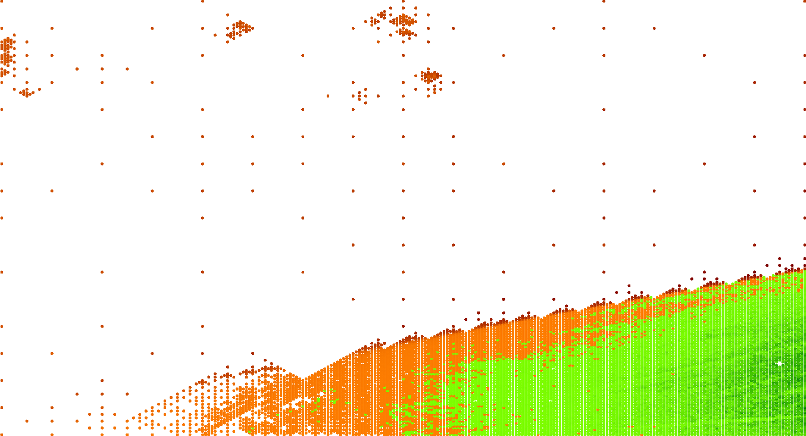
\includegraphics[width=0.9\textwidth]{1.0.0.Final/analysis1.png}}
	\end{subfigure}
	\begin{subfigure}[b]{0.3\textwidth}
		\fbox{
\includegraphics[width=0.9\textwidth]{1.0.0.Final/analysis2.png}}
		\centering
	\end{subfigure}
	\begin{subfigure}[b]{0.3\textwidth}
		\centering
		\fbox{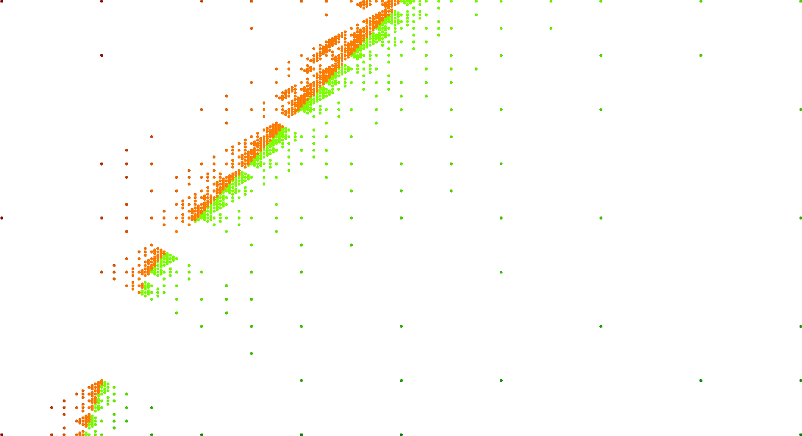
\includegraphics[width=0.9\textwidth]{1.0.0.Final/analysis3.png}}
	\end{subfigure}
	\caption{Ukázka vizualizace výsledku analýzy několika modelů. Zelené body označují hodnoty, kde daná vlastnost platí, v červených bodech vlastnost naopak neplatí.}
\end{figure}

\section{Čtvrtá etapa}

Ve čtvrté etapě, probíhající od začátku do konce listopadu, jsme pracovali na dokončení grafického rozhraní a
optimalizaci výpočtu, který se již v této etapě prováděl paralelně. Z hlediska optimalizace šlo zejména o:

\begin{itemize}
	\item	odstranění duplicitních výpočtů, zejména zlepšíním práce cache, ve které se ukládají již odsimulované trajektorie,
	\item	odstranění referencí na data již nepotřebných odsimulovaných trajektorií, aby mohla být zpracována pomocí \textit{garbage collectoru}.
\end{itemize}

Vydaná verze z~konce čtvrté etapy je k~dispozici na stránkách našeho projektu\footnote{\url{https://github.com/sybila/parasim/zipball/1.0.0.M4}},
kde najdete též seznam vyřešených úkolů\footnote{\url{https://github.com/sybila/parasim/issues?milestone=6&state=closed}}.

\section{Pátá etapa}

V páté etapě, probíhající od začátku do konce prosince, jsme pracovali na vydání finální verze aplikace, psaní testů a dokumentace\footnote{\url{https://github.com/sybila/parasim/wiki}}.
Dále jsme se zaměřili na: 

\begin{itemize}
	\item	spuštění analýzy nad dalšími reálnými modely,
	\item	přidání globální robustnosti do analýzy,
	\item	zjednodušení nastavení analýzy (bylo odstraněno nastavení pro počáteční rozdělení prostoru iniciálních hodnot).
\end{itemize}

\begin{figure}[h!]
	\centering
	\begin{subfigure}[b]{0.48\textwidth}
		\centering
		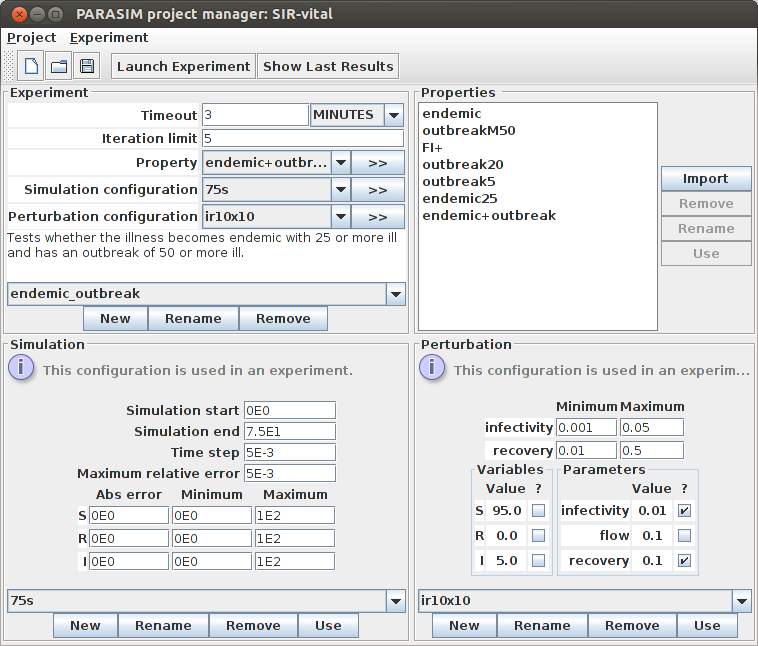
\includegraphics[width=0.8\textwidth]{1.0.0.Final/project-manager.png}
		\caption{Manažer pro správu.}
	\end{subfigure}
	\begin{subfigure}[b]{0.48\textwidth}
		\centering		
		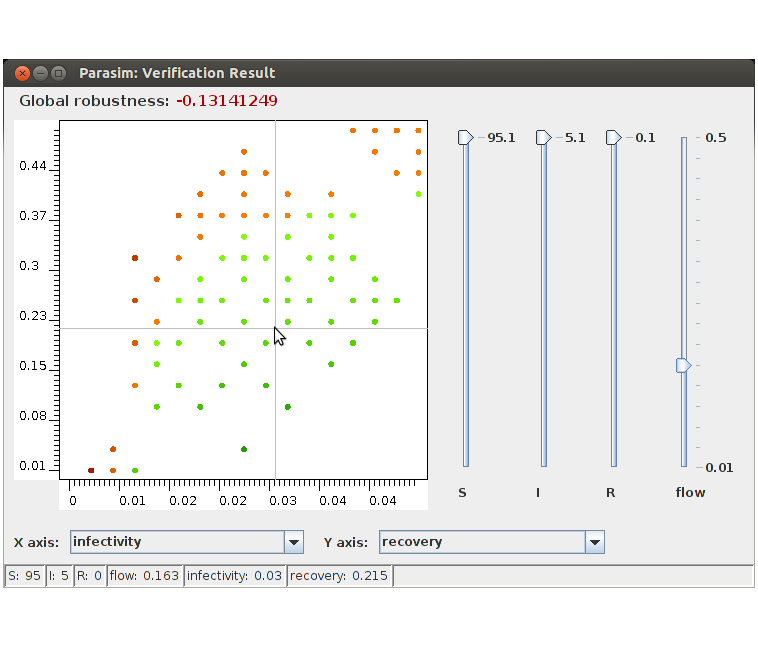
\includegraphics[width=0.8\textwidth]{1.0.0.Final/plotter.png}
		\caption{Komponenta pro vizualizaci výsledků analýzy.}
	\end{subfigure}
	\caption{Screenshoty z aplikace s grafickým rozhraním.}
\end{figure}

Finální verze z konce páté etapy je k~dispozici na stránkách našeho projektu\footnote{\url{https://github.com/sybila/parasim/zipball/1.0.0.Final}},
kde najdete též seznam vyřešených úkolů\footnote{\url{https://github.com/sybila/parasim/issues?milestone=3&page=1&state=closed}}.

\section{Shrnutí}

Byl vytvořen nástroj pro analýzu dynamických systémů modelovaných pomocí
obyčejných diferenciálních rovnic. Na rozdíl od existujících nástrojů pro simulaci chování
dynamických systémů a monitoring temporálních vlastností nad běhy těchto systémů byl kladen důraz
na modulární architekturu, jež umožňuje budoucí vývoj a testování
optimalizace a paralelizace jednotlivých modulů i analytických algoritmů.

Nástroj se skládá z aplikace s grafickým rozhraním pro správu modelů, vlastností a nastavení analýzy
a aplikace pro příkazovou řádku vhodné zejména pro dávkové spouštění. Obě aplikace umí spustit analýzu
a zobrazit její výsledek, to i v případě, že se jedná o vícerozměrná data.

Repozitář projektu obsahuje reálné modelů s přiloženými vlastnostmi a nastaveními analýzy,
nad kterými byl nástroj vyzkoušen. Kdokoliv si může analýzu nad těmito modely pustit sám, modely
a vlastnosti dále rozšiřovat, případně přidávat další.

Během řešení projektu se objevilo několik cest, kterými by se mohl ubírat další vývoj. Zejména se jedná o:

\begin{itemize}
	\item	vytvoření webovou službu zpřístupňující analýzu online,
	\item	použítí rychlejších nástrojů pro řešení obyčejných diferenciálních rovnic \footnote{momentálně je použit Octave, \url{http://octave.sourceforge.net/}},
	\item	zahrnutí projekce do vizualizace výsledků analýzy.
\end{itemize}

\end{document}

